\documentclass{beamer}

\usepackage[ngerman]{babel}
\usepackage[utf8]{inputenc}
\usepackage[T1]{fontenc}
\usepackage{lmodern}
\usepackage{pdfpages}

\usetheme{Boadilla}  %% Themenwahl
\usecolortheme{whale}


%% Variables. You may want to change them. 
\title{Campusrallye - Tutoreinteilung}
\subtitle{}
\author{}
\date{\today}

\setbeamertemplate{headline}
{
  \leavevmode%
  \hbox{%
  \begin{beamercolorbox}[wd=\paperwidth,ht=8.25ex,dp=1.5ex]{palette secondary}
    \raggedright
    \hspace*{2em}%
    
\includegraphics[width=15mm]{media/fachschaft.png} 
    \hspace{100pt}
\includegraphics[width=5mm]{media/fakultaet_mathe.png}
    \hspace{10pt}
\includegraphics[width=5mm]{media/fakultaet_physik.png}
    \hspace{10pt}
\includegraphics[width=5mm]{media/fakultaet_informatik.png}
    \hspace{100pt}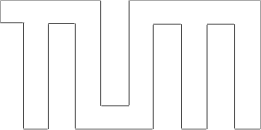
\includegraphics[width=10mm]{media/tum.png}
    \hspace*{2em}%
  \end{beamercolorbox}%
  }%
}


% If you want to get rid of the presentation controls in the bottom right corner, enable this setting
% \setbeamertemplate{navigation symbols}{} 

% This setting removes the footer but keeps the frame (=slide) number in the bottom right corner
% \setbeamertemplate{footline}[frame number]{}

% This setting removes the footer completely. It is going to override footer-related settings from above!
% \setbeamertemplate{footline}{}

%%%%%%%%%%%%%%%%%%%%%%%%%%%%%%%%%%%%%%%%%%%%%%%%%%%%%%%%%%%%%%%%%%%%%%%%%%%%%%%%%%%%%%%%%%%%%%%%%%%%%%%%%%%%%%%%%%%%%%%
% The content starts here
\begin{document}


	
	% First page
	\maketitle
	% Comment this out to remove the table of contents
	
	\begin{frame}
		\huge
		\center
		\frametitle{Hinweise}
		
		\begin{itemize}
			\item 53 Tutoren
			\item 21 Stationen + Infostand + Getränkeverkauf 
			\item >= 1 Handy mit vollem Akku dabei haben!
		\end{itemize}
	\end{frame}
	
	
	
	\begin{frame}
		\huge
		
		\frametitle{Timetable}
		Samstag 14.10.2018\\
		
		\begin{itemize}
			\item 10:15 Uhr: Treffpunkt \normalsize im Raum 00.07.14 \huge
			\item 11:00 - 14:00 + x: Rallye 
			\item ca 15:00 Uhr: Siegerehrung
		\end{itemize}
	\end{frame}
	
	
	
	
	\begin{frame}
		\huge
		\begin{center}
			Anmeldung auf: \\
			\url{https://bit.ly/2y9Apg0} \\ \ \\
		
		\end{center}
		\large
		\begin{itemize}
			\item Meldet euch mit richtigem Namen an!
			\item Installiert die App auf eurem Handy!
			\item Eine Liste der Stationen ist ab Freitag zu finden.
			\item Ihr könnt uns dort bit Samstag Abend mitteilen, welche Station ihr übernehmen wollt.
			\item Meldet euch gerne als Zweiergruppen.
			\item FCFS!
		\end{itemize}
		
	\end{frame}
	%Diagramm über den Fakt, dass Übung sehr wichtig ist?!
	
	% Sections are like chapters and used to structure the presentation 

\end{document}
